\documentclass[sans,mathserif]{beamer}
%handout,notes=show

%\usepackage{pgfpages}
%\pgfpagesuselayout{8 on 1}[a4paper,border shrink=5mm]

\usetheme{default}
\usepackage{fp}
\usepackage[thicklines]{cancel}
\usepackage{tikz}
\usepackage{multirow}
\usepackage{amsmath}
\usepackage{ifthen}
\usepackage{animate}
\usepackage{setspace}
\usepackage{forloop}
%\usepackage{concmath}
%\usepackage{pxfonts}
%\usepackage{eulervm}
%\usepackage{mathpazo}
%\renewcommand\mathfamilydefault{\rmdefault}

%\usefonttheme{professionalfonts}
%\setmathfont{}
%\setsansfont{Palatino}
\usetikzlibrary{arrows,backgrounds,positioning,fit,chains,shapes,calc}

%\usepackage{handoutWithNotes}
%\pgfpagesuselayout{4 on 1 with notes}[a4paper,border shrink=5mm]

\setbeamertemplate{navigation symbols}{}

\title{Basics of modern computers}
\author{Dag Sverre Seljebotn}
%\institute{Department of Mathematics \\ University of Oslo}
\date{September 7, 2012}

\newcommand{\V}{\vskip1em}

\setbeamersize{sidebar width left=0cm, sidebar width right=0cm}
\setbeamersize{text margin left=.8cm, text margin right=.8cm}

\defbeamertemplate{note page}{infolines}
{%
  \vskip3em
%  \setstretch{1.8}
  \Large
  \rmfamily
  \insertnote
}
\setbeamertemplate{note page}[infolines]

\renewcommand{\CancelColor}{\color{red}}


\begin{document}


\begin{frame}
  \titlepage
\end{frame}

\begin{frame}{Memory, encoding and pointers}
  \begin{center}
  von Neumann architecture: CPU $\leftrightarrow$ memory bus $\leftrightarrow$ memory

~

    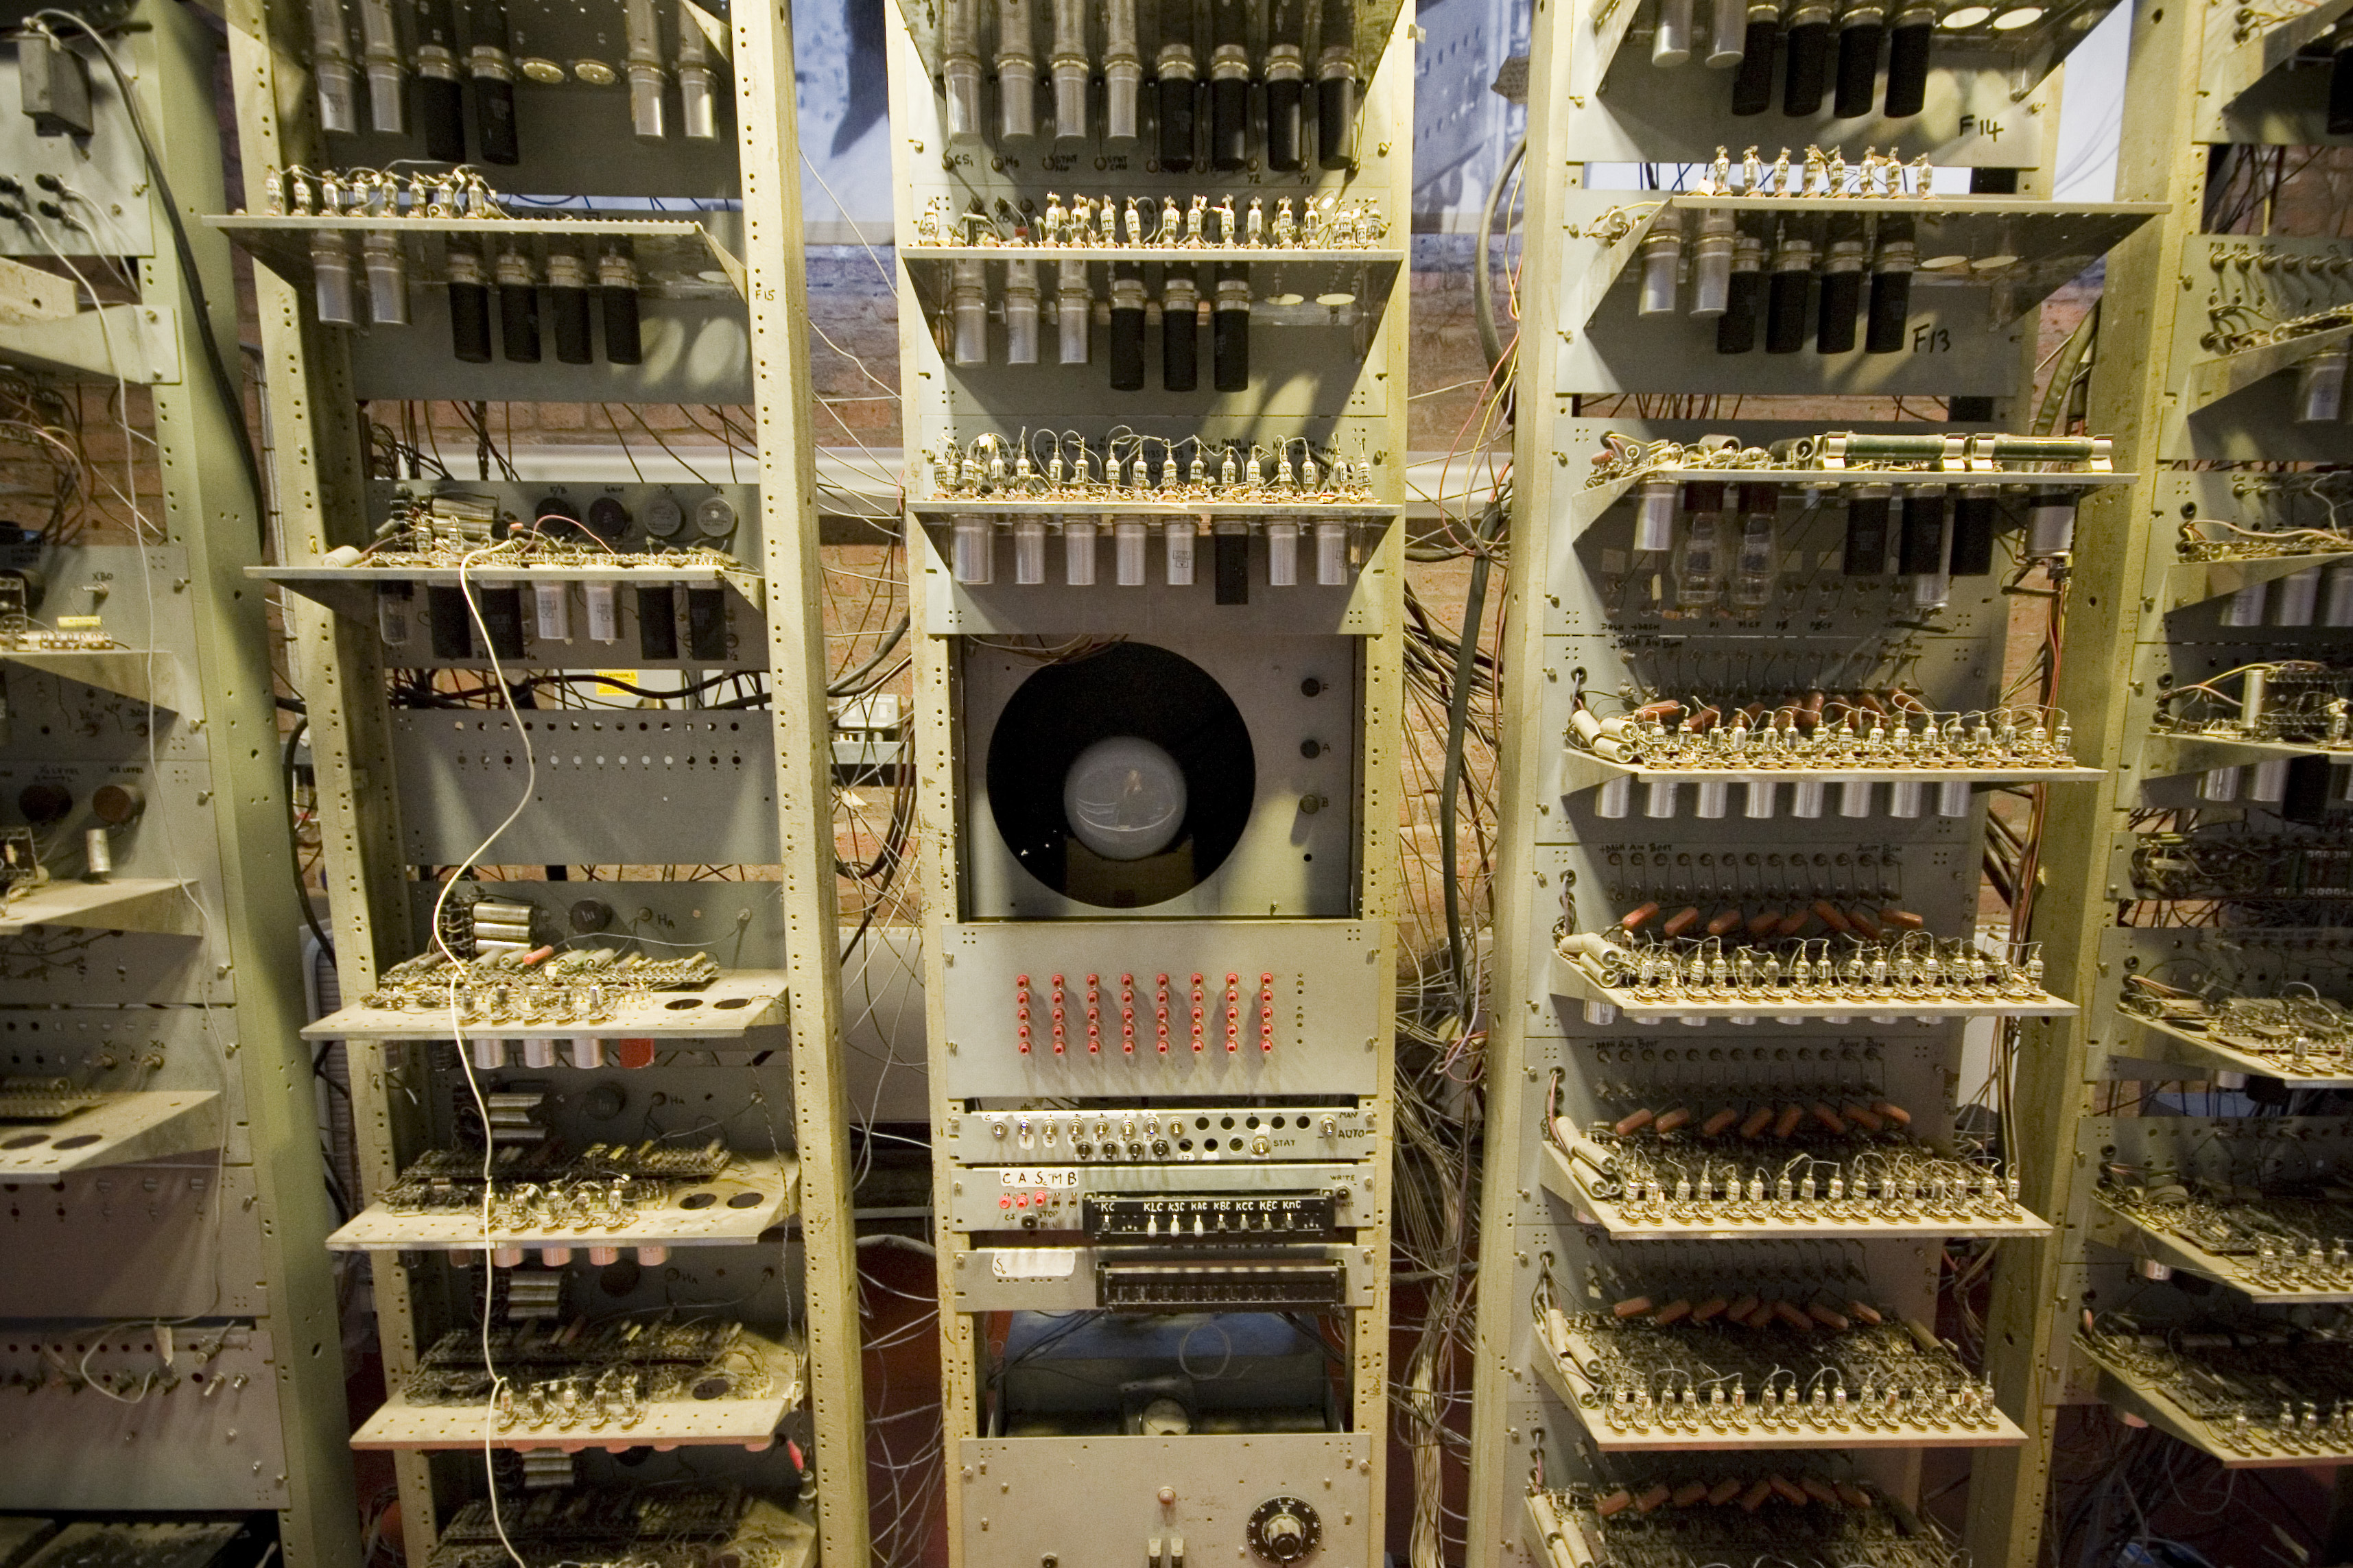
\includegraphics[width=0.7\textwidth]{SSEM.jpg}\\
    Manchester Small-Scale Experimental Machine, world's first
    stored-program computer (1948)
  \end{center}
\end{frame}

\newcommand{\bs}[3]{{\color{blue}#1} \cdot {#2}^{#3} }
\newcommand{\br}[3]{{\color{red}#1} \cdot {#2}^{#3} }
\begin{frame}{Memory, encoding and pointers}

  Everything (data, program) is encoded in {\em memory bytes},
  which (nowadays) are always 8 bits, allowing $2^8=256$ distinct values.

%124     124    0x7c   |    01111100 
{\small
  \begin{align*}
    124_{10} &= \bs{1}{10}{2} + \bs{2}{10}{1} + \bs{4}{10}{0} \\
    &= \bs{0}{2}{7} + \bs{1}{2}{6} + \bs{1}{2}{5}
              + \bs{1}{2}{4} + 
              \only<1>{\bs{1}{2}{3} + \bs{1}{2}{2} + \bs{0}{2}{1} + \bs{0}{2}{0}}
              \only<2>{\br{1}{2}{3} + \br{1}{2}{2} + \br{0}{2}{1} + \br{0}{2}{0}}
              \\
\uncover<2->{
 &= \bs{7}{16}{1} + \br{12}{16}{0} = \text{\tt 0x7c}}
  \end{align*}
}

  Demo: {\tt binary.c}
\end{frame}

\begin{frame}{Pointers}

TODO: Example in C of using pointers
  
\end{frame}

\begin{frame}{Virtual memory}
  \begin{tikzpicture}
    \node at (0,0) {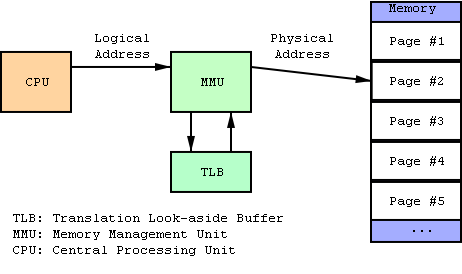
\includegraphics[width=.35\textwidth]{mmu.png}};
    \node at (6,-2) {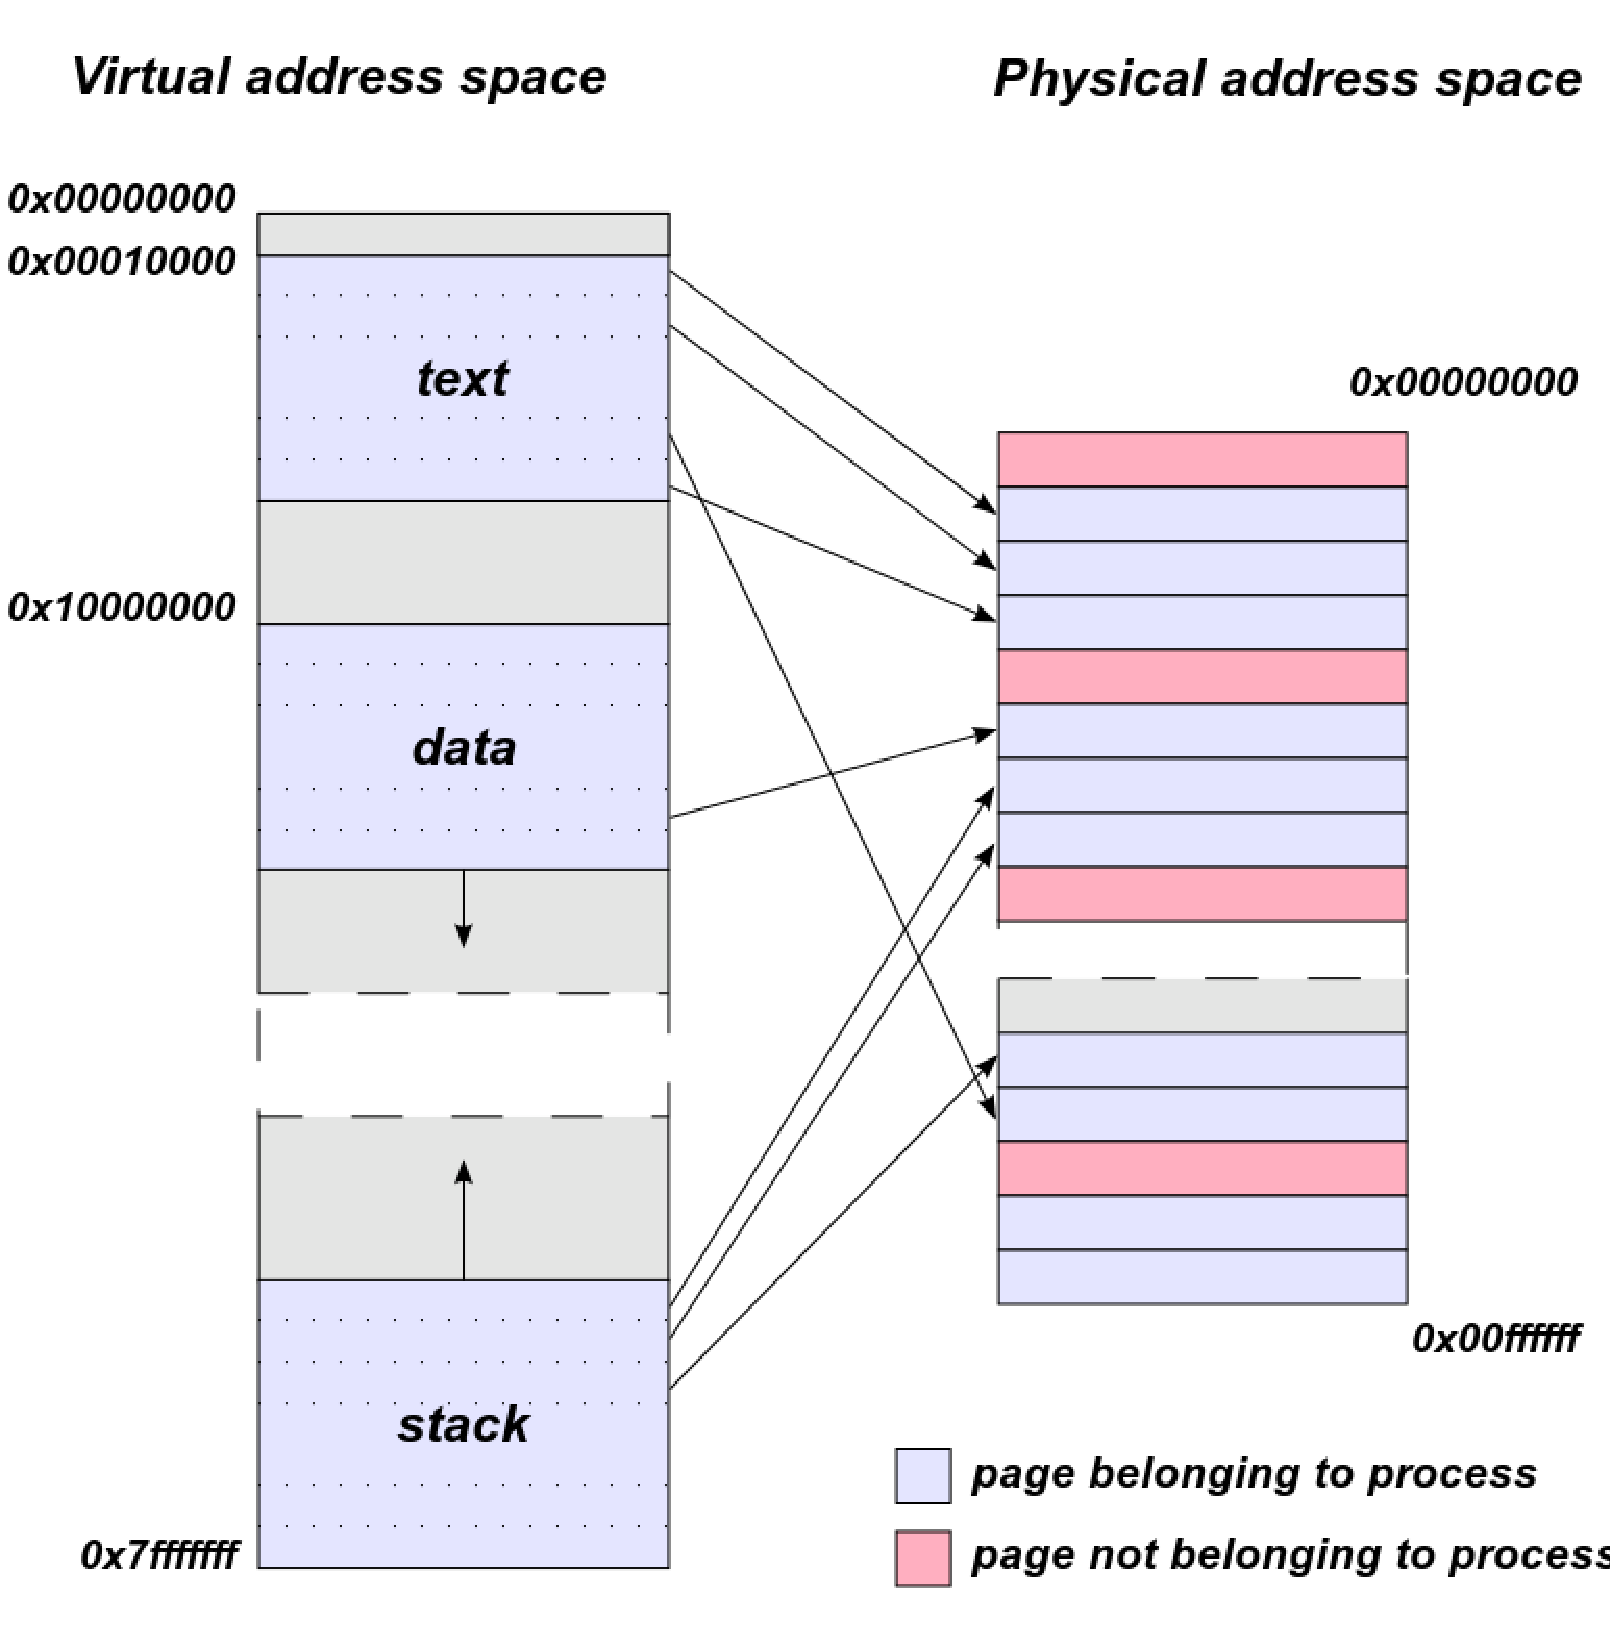
\includegraphics[width=.6\textwidth]{virtualmemory.pdf}};
  \end{tikzpicture}
{\tiny Illustrations from Wikipedia}
\end{frame}


\begin{frame}{Ways of using memory}

\uncover<+->{Conventionally we divide memory into:}
  \begin{itemize}
  \item<+-> {\bf Static}: Your program, global variables, constants
  \item<+-> {\bf Heap}: Dynamically allocated/deallocated blocks
    \begin{itemize}
    \item C: {\tt malloc()}, {\tt free()} functions
    \item C++: {\tt new}, {\tt delete} keywords
    \item Fortran: {\tt allocate}, {\tt deallocate} keywords
    \item Modern languages: {\tt new} + Garbage Collection
    \end{itemize}
  \item<+-> {\bf Stack}: Allocated at program startup
    \begin{itemize}
    \item Implicitly used through program flow
    \end{itemize}
  \end{itemize}

~

\uncover<4->{Demo program: {\tt knapsack.c} }

\end{frame}


\begin{frame}{Simple model of CPU}
  Loads, registers, etc.; some simple assembly
\end{frame}



\begin{frame}{Benchmarking}
\uncover<+->{Issues:}

\begin{itemize}
\item<+-> What speed is your CPU {\em really} running at?
  \begin{enumerate}
  \item Power saving
  \item ``Turbo mode''
  \end{enumerate}

\item<+-> Interruptions from the OS
\item<+-> Benchmark the CPU only, or the entire system?
\end{itemize}

\uncover<+->{One strategy (out of many):}
\begin{itemize}
%\item<+-> test
\item<+-> Benchmark using all CPU cores
\item<+-> Take many samples of {\em wall time}, then use {\em minimum}
\item<+-> For each sample, may have to repeat and average
\end{itemize}

\end{frame}

\begin{frame}{Memory bandwidth and latency}
  
\end{frame}

\begin{frame}
  \begin{center}
    \LARGE A more complicated picture of CPUs
  \end{center}
\end{frame}

\begin{frame}{CPUs getting more complicated}
  \begin{center}
    \only<1>{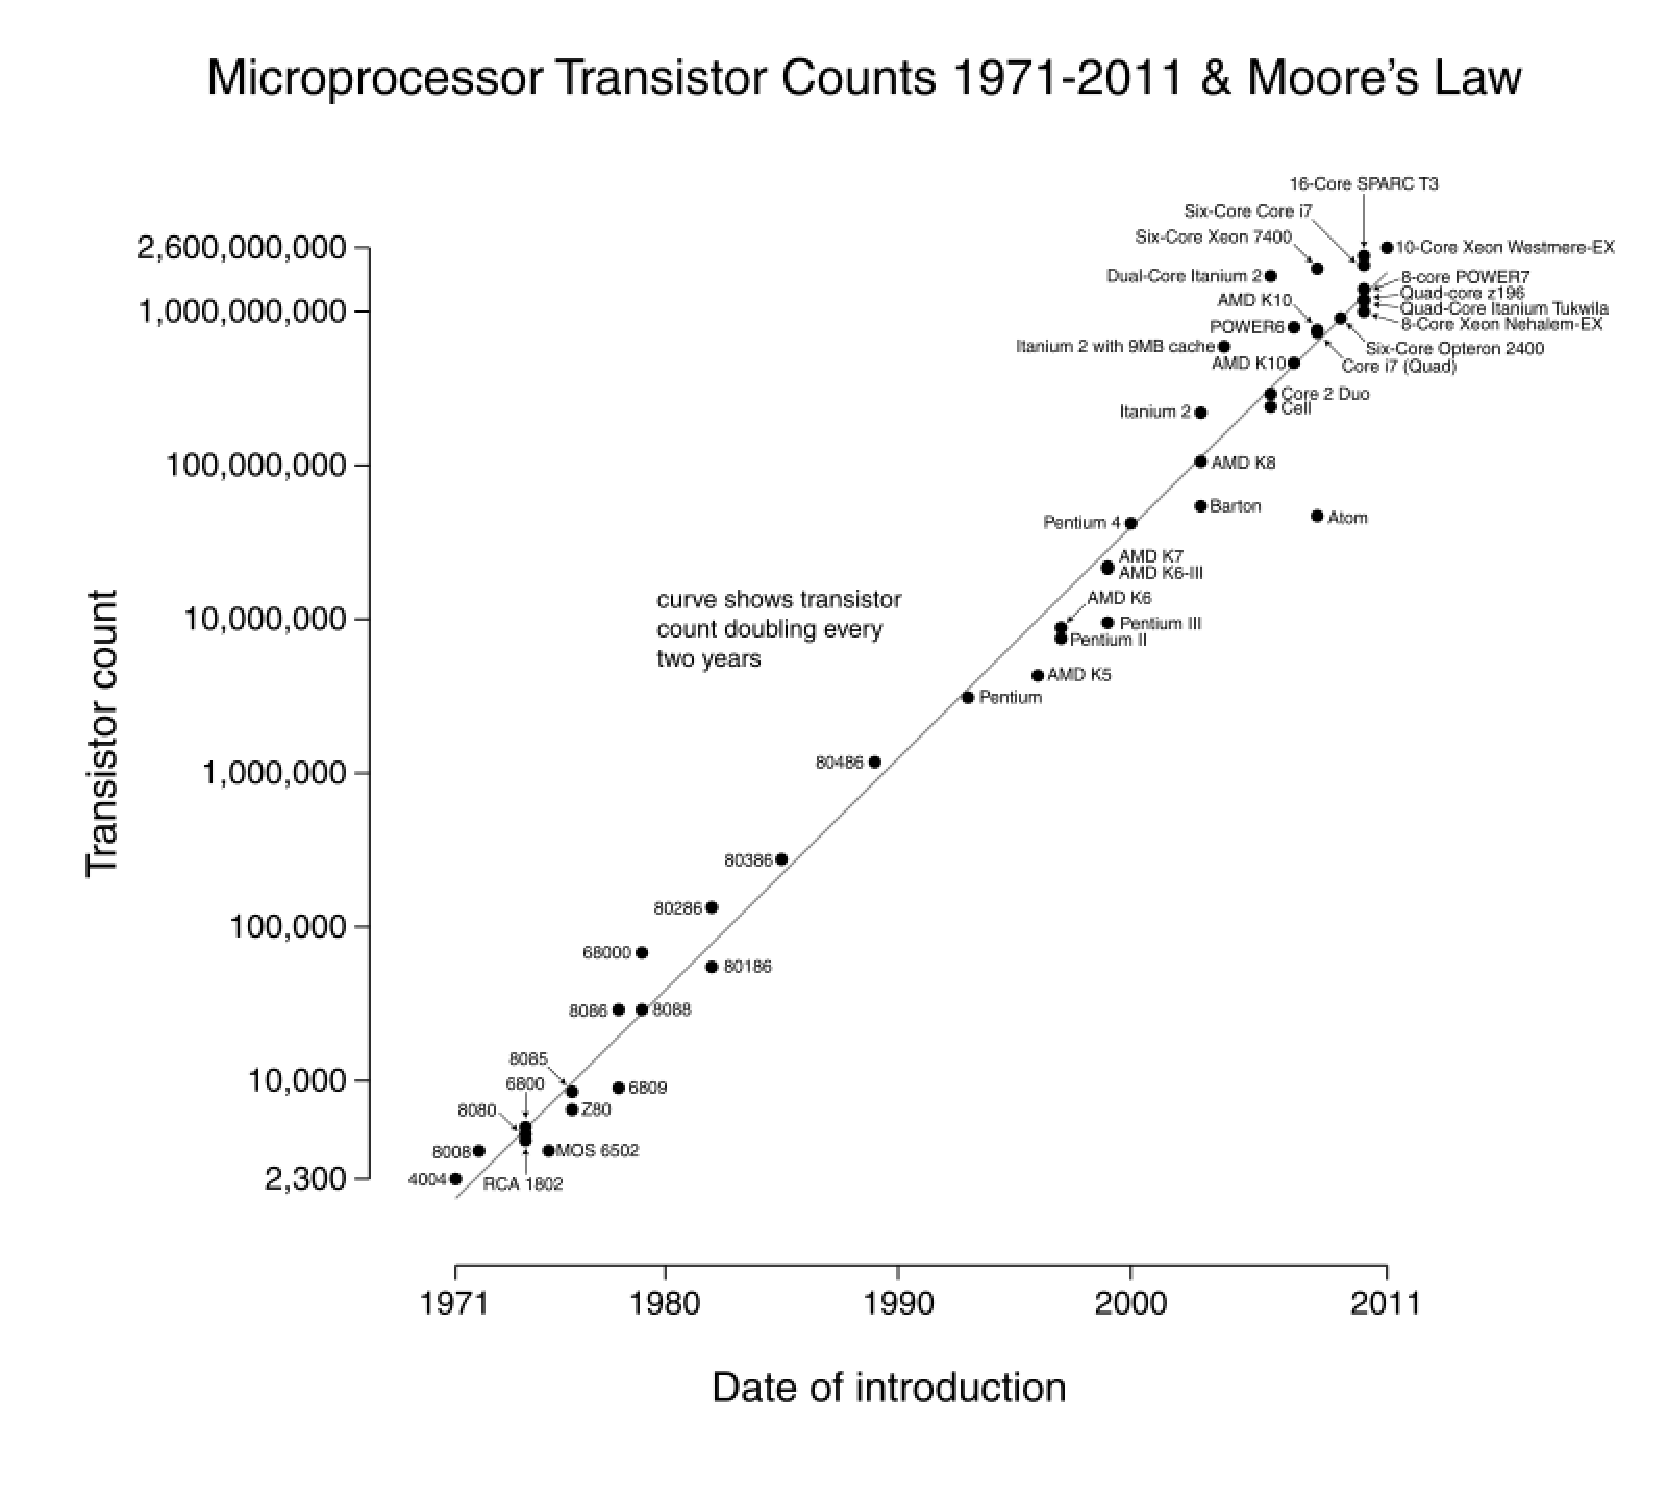
\includegraphics[width=0.8\textwidth]{transistors.pdf}}
    \only<2>{But:\\[5mm]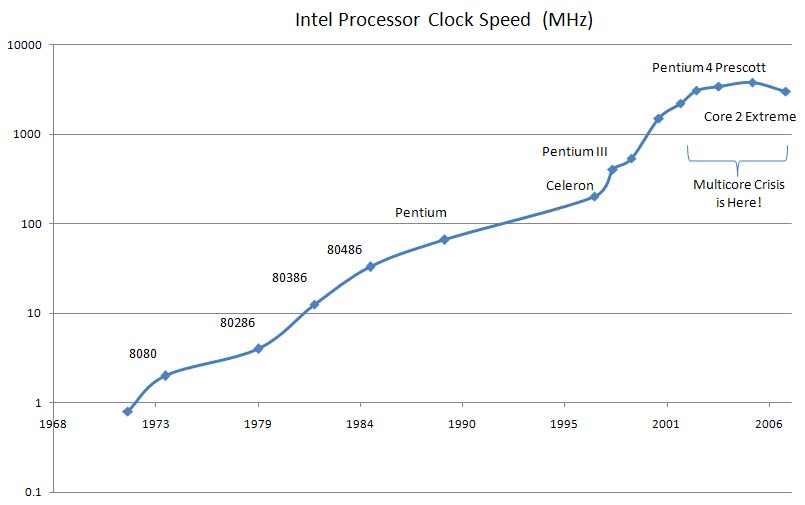
\includegraphics[width=0.8\textwidth]{clockspeeds.jpg}}
  \end{center}
  
\end{frame}

\begin{frame}{CPUs today}
  \begin{center}
    \only<1>{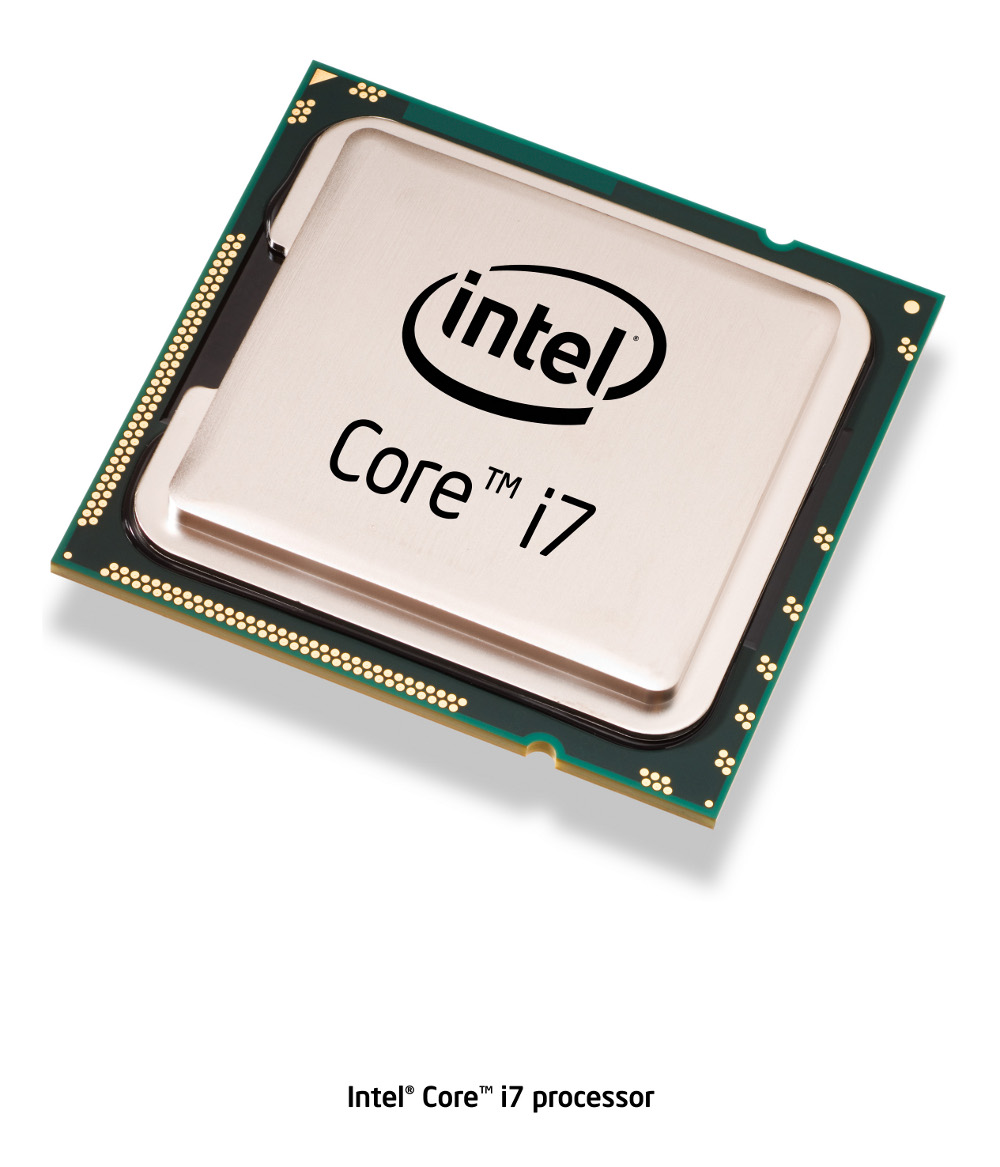
\includegraphics[width=0.8\textwidth]{nehalem_front.jpg}}
    \only<2>{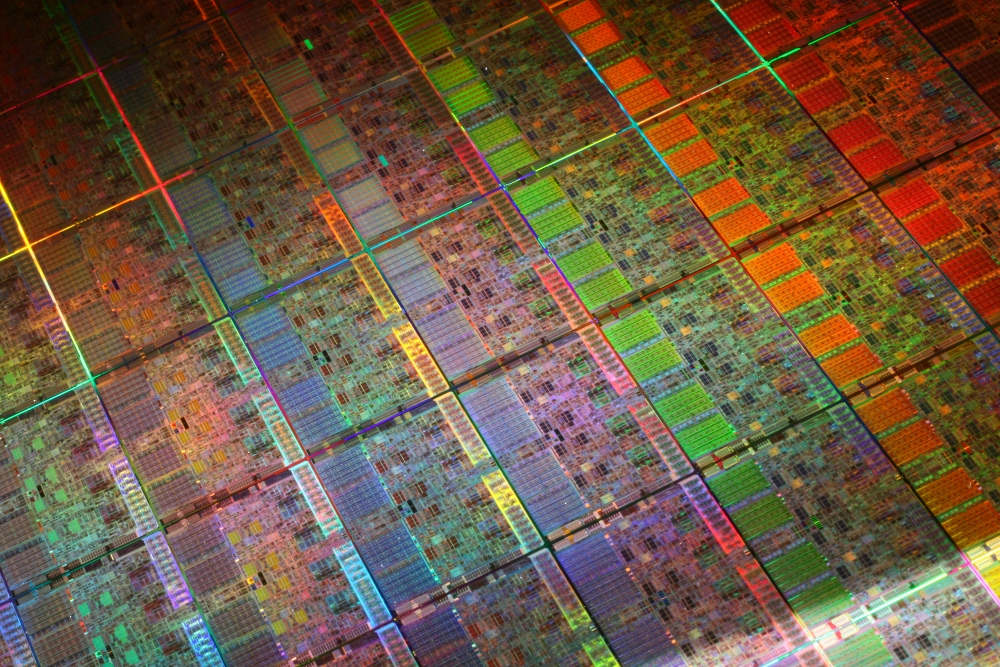
\includegraphics[width=0.8\textwidth]{nehalem_wafer.jpg}}
    \only<3>{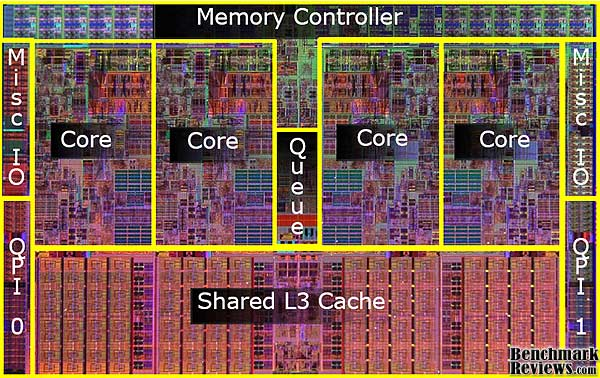
\includegraphics[width=0.8\textwidth]{nehalem_callout.jpg}}
    \only<4>{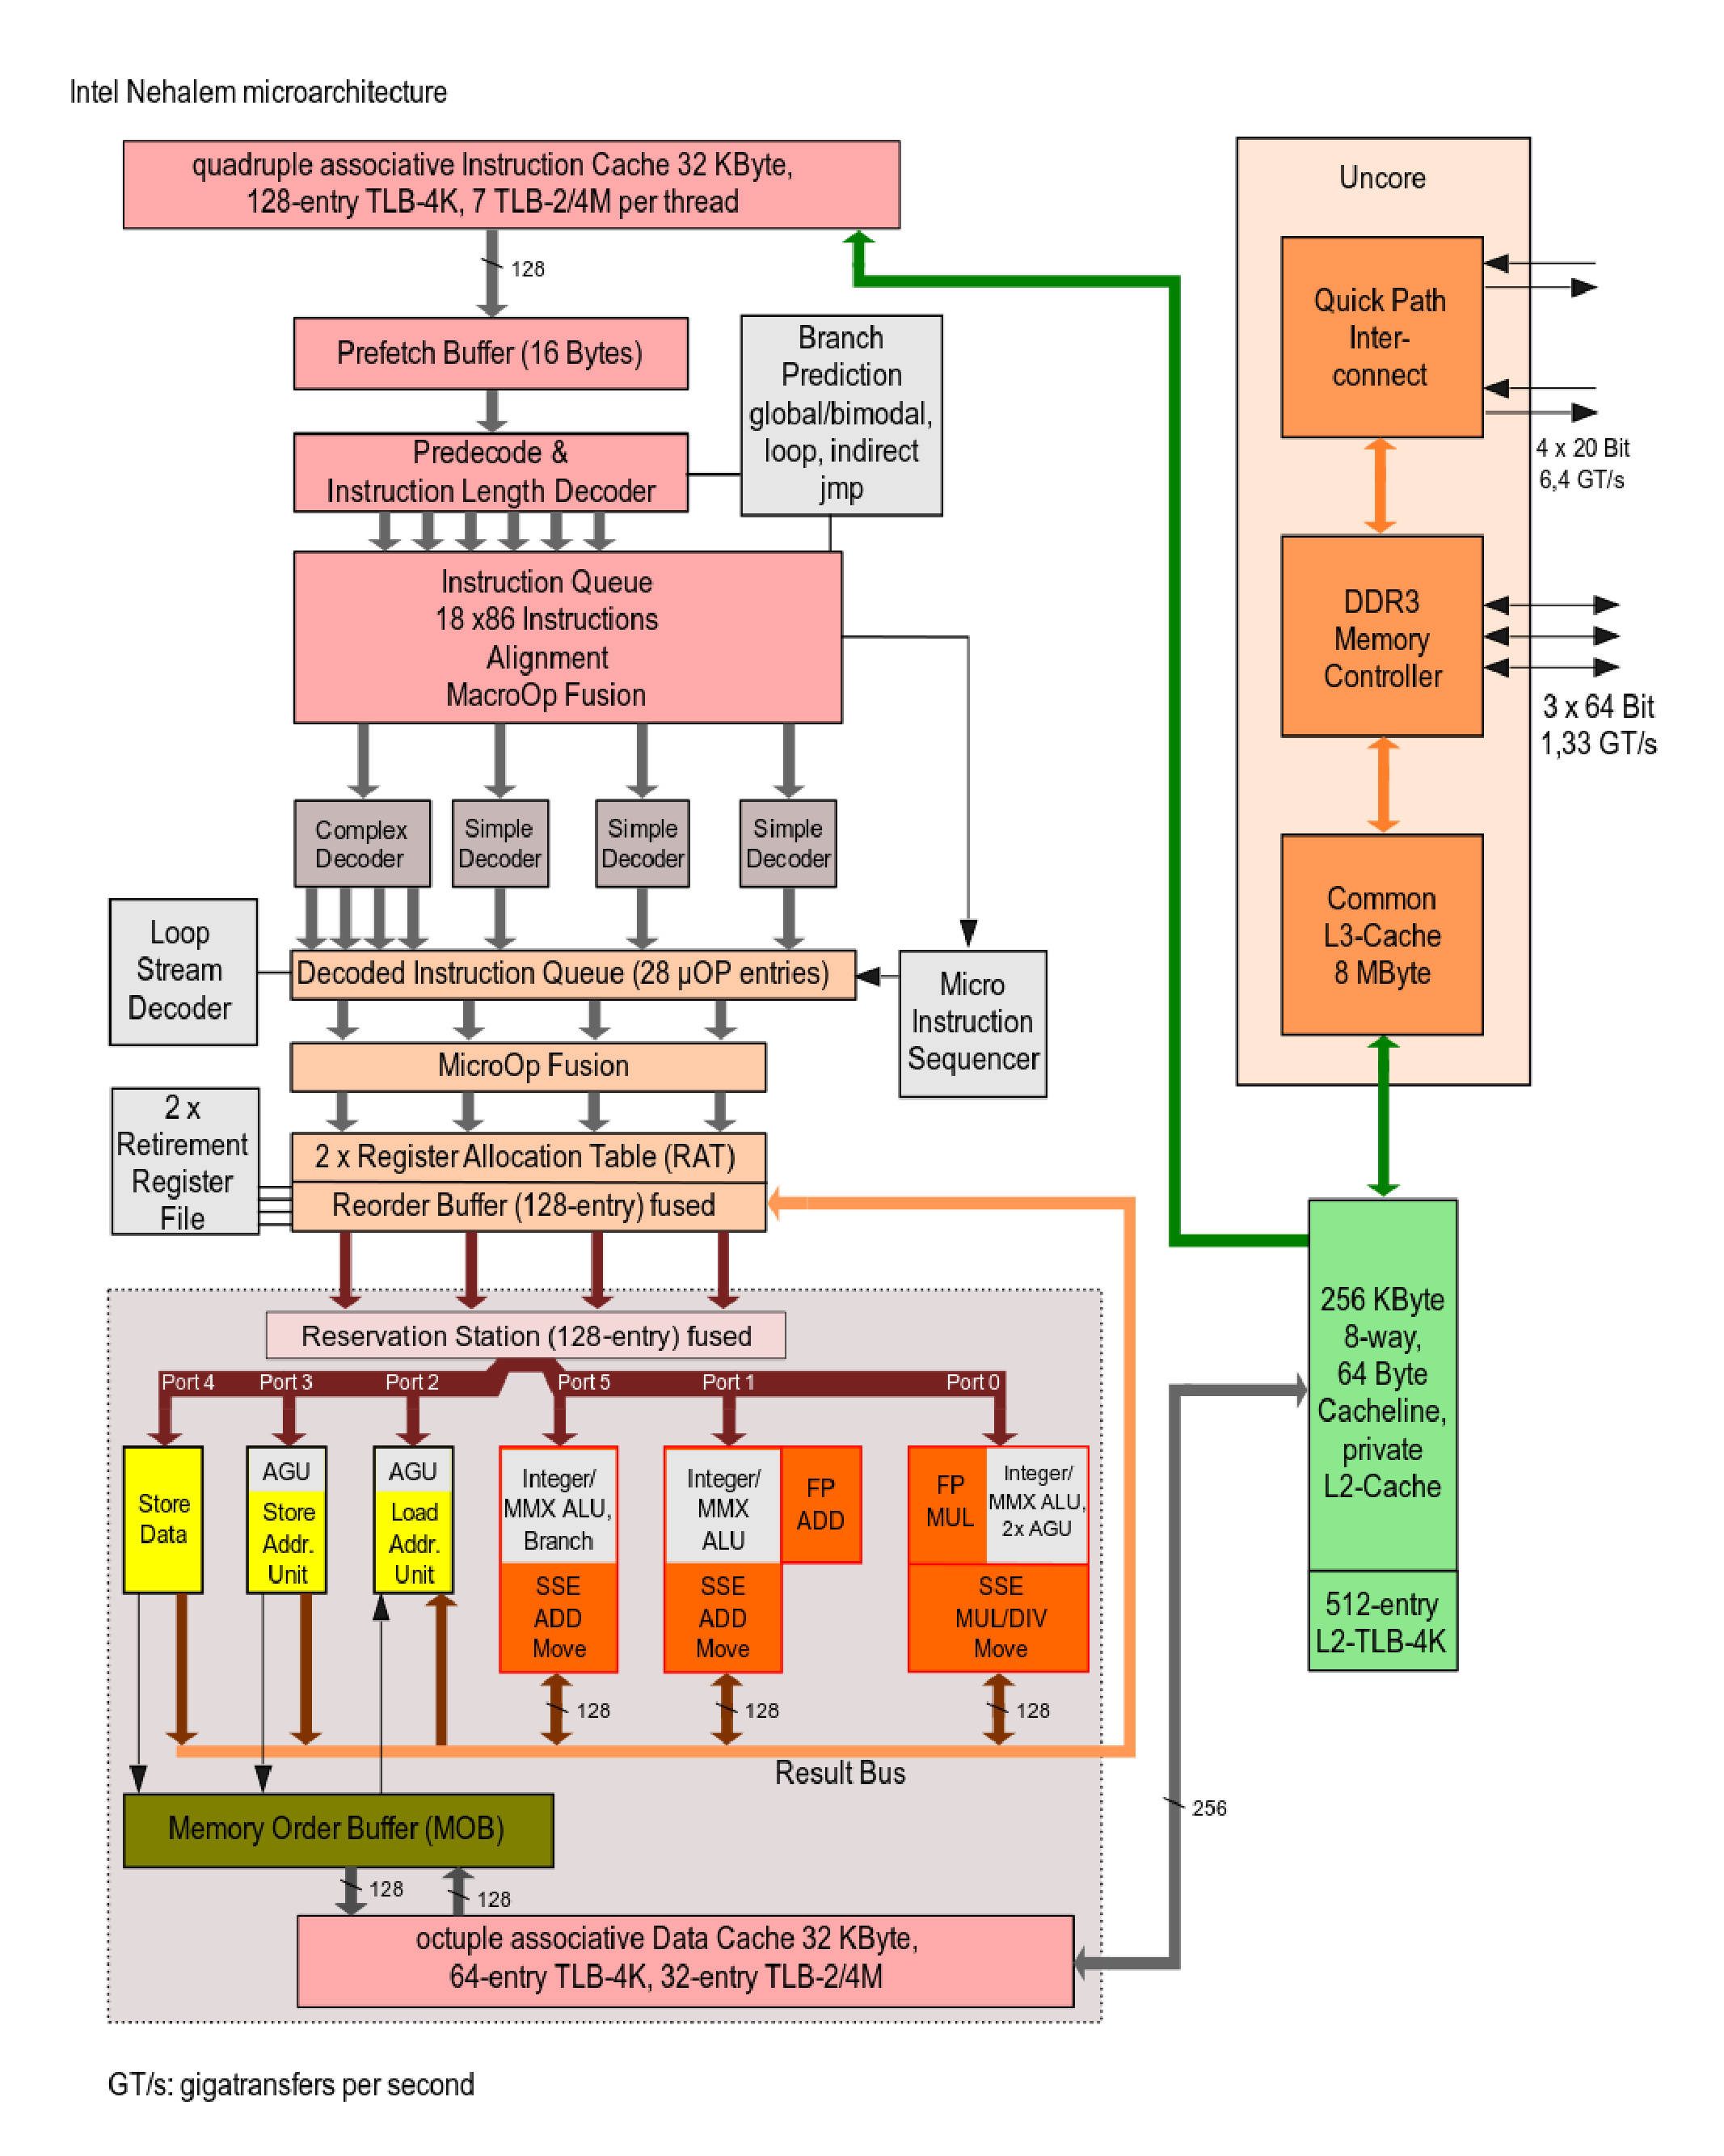
\includegraphics[width=0.6\textwidth]{nehalem_arch.pdf}}
  \end{center}
\end{frame}


\end{document}